Chương này,  trình bày một số nội dung về dữ liệu và những công cụ được sử dụng trong quá trình thực nghiệm. Đánh giá kết quả thực nghiệm đã làm được cũng như khả năng ứng dụng và hướng phát triển của đề tài trong tương lai. Qua đó đưa ra những nhận xét, đánh giá và kết luận chung cho đề tài.

\section{Dữ liệu thực nghiệm}
Để tiến hành làm thực nghiệm những nội dung nghiên cứu trong đề tài, tôi đã sử dụng hai nguồn dữ liệu chính để làm thực nghiệm. Một nguồn là dữ liệu của trò chơi Code Hunt, nguồn dữ liệu còn lại do tôi tự thiết kế.

Code Hunt \cite{CodeHunt} là một game về lập trình, được sử dụng cho các cuộc thi viết mã và thực hành các kỹ năng lập trình do Microsoft phát triển. Code Hunt dựa trên công cụ Pex, ứng dụng kỹ thuật DSE khám phá các nhánh đường đi của chương trình để suy ra giá trị đầu vào có độ phủ cao. Mã Code Hunt là một được xử lý trực tuyến, trong đó mỗi câu đố được trình bày như một bài kiểm tra. Người chơi phải chọn câu hỏi và trả lời mã câu hỏi bằng cách viết một đoạn mã sao cho kết quả trùng với kết quả cử câu hỏi. Hiện Code Hunt đã được hơn 350.000 người chơi sử dụng tính đến tháng 8 năm 2016. Dữ liệu từ các cuộc thi gần đây đã được công khai và cho phép những người quan tâm đến Code Hunt tải về để phân tích và nghiên cứu trong cộng đồng giáo dục.

\label{sec:data}
\begin{center}
	\begin{figure}[h]
		\begin{center}
			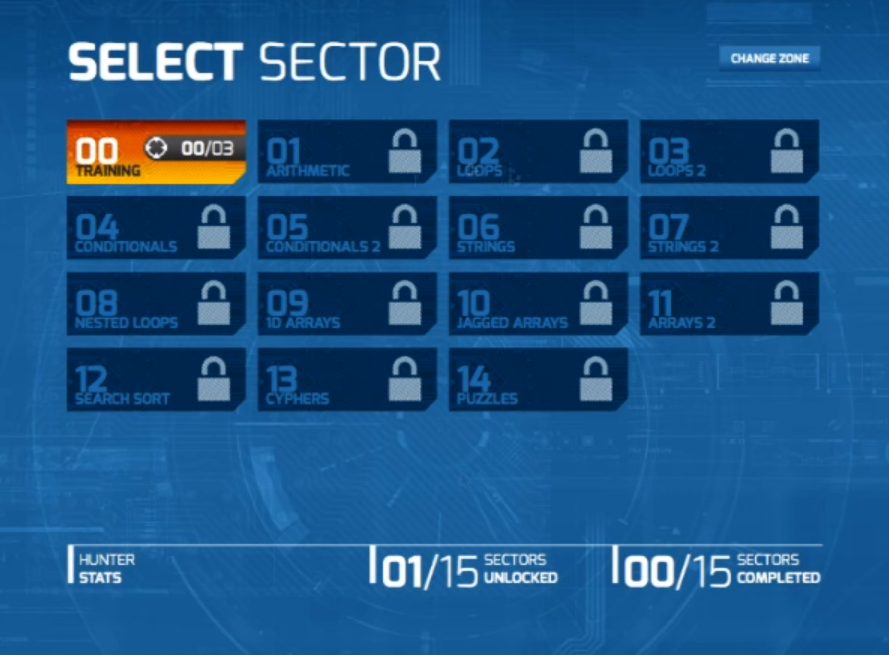
\includegraphics[scale=.3]{codehunt2.png}
		\end{center}
		\caption{Giao diện viết chương trình của Code Hunt}
		\label{refhinh1}
	\end{figure}
\end{center}

Tập dữ liệu Code Hunt là một tập dữ liệu chứa các chương trình do sinh viên trên toàn thế giới viết, với 250 người sử dụng, 24 câu hỏi và khoảng 13.000 chương trình được sinh viên thực hiện trên 2 ngôn ngữ là Java và C\#. Để có thể sử dụng tập dữ liệu Code Hunt cho đề tài của tôi, tôi đã thực hiện chuyển đổi những chương trình sử dụng ngôn ngữ lập trình Java thành ngôn ngữ C\# bằng công cụ chuyển đổi của hãng Tangible Software Solutions, loại bỏ một số chương trình lỗi và không phù hợp với đề tài.

\begin{center}
	\begin{figure}[h]
		\begin{center}
			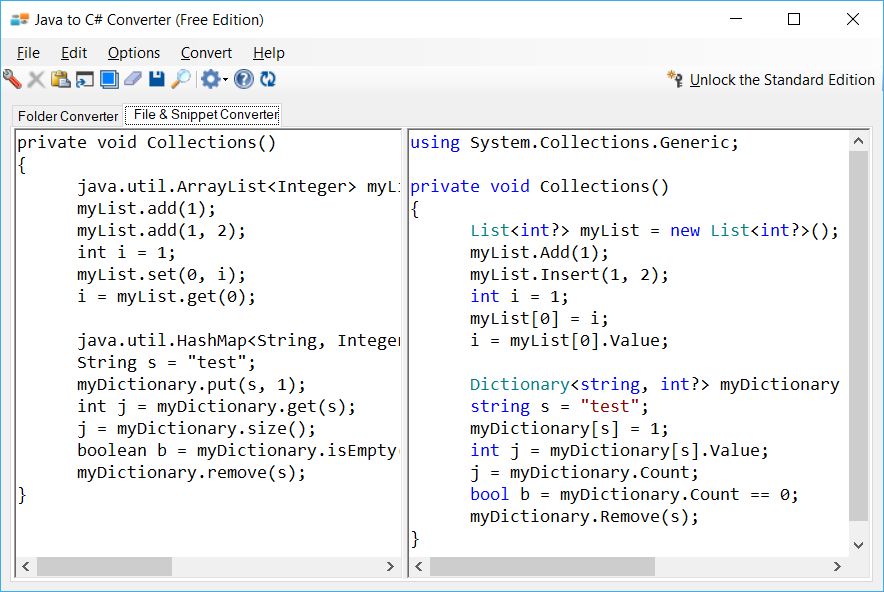
\includegraphics[scale=.4]{java-to-csharp-collections.png}
		\end{center}
		\caption{Chuyển đổi code Java sang C\#}
		\label{refhinh1}
	\end{figure}
\end{center}

\section{Công cụ dùng trong thực nghiệm}
%Phần này trình bày những công cụ được sử dụng để triển khai thực nghiệm như: công cụ sinh dữ liệu kiểm thử, môi trường lập trình, \dots

Trong quá trình làm thực nghiệm, tôi đã sử dụng một số công cụ để làm ví dụ minh hoa cho các kỹ thuật đo độ tương tự hành vi của chương chình, cụ thể như sau:

\subsection*{Microsoft Visual studio}
Microsoft Visual Studio là một môi trường phát triển tích hợp từ Microsoft. Nó được sử dụng để phát triển chương trình máy tính cho Microsoft Windows, cũng như các trang web, các ứng dụng web và các dịch vụ web. Microsoft Visual Studio sử dụng nền tảng phát triển phần mềm của Microsoft như Windows API, Windows Forms, Windows Presentation Foundation, Windows Store và Microsoft Silverlight. 

\begin{center}
	\begin{figure}[h]
		\begin{center}
			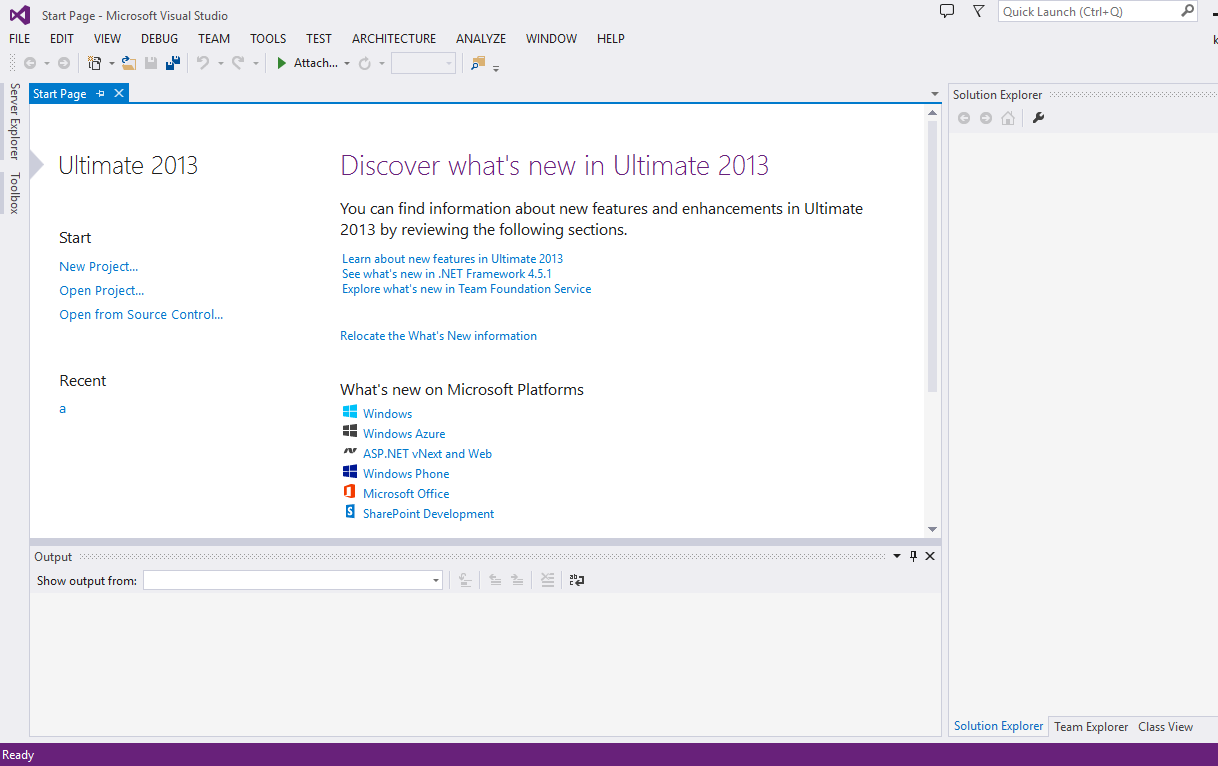
\includegraphics[scale=.3]{visualstudio.png}
		\end{center}
		\caption{Giao diện phần mềm Visual studio 2013}
		\label{refhinh1}
	\end{figure}
\end{center}

Visual Studio hỗ trợ nhiều ngôn ngữ lập trình khác nhau và cho phép trình biên tập mã và gỡ lỗi để hỗ trợ (mức độ khác nhau) hầu như mọi ngôn ngữ lập trình. Các ngôn ngữ tích hợp gồm có C, C++ và C++/CLI (thông qua Visual C++), VB.NET (thông qua Visual Basic.NET), C\#  (thông qua Visual C\#) và F\# (như của Visual Studio 2010). Hỗ trợ cho các ngôn ngữ khác như J++/J\#, Python và Ruby thông qua dịch vụ cài đặt riêng rẽ. Nó cũng hỗ trợ XML/XSLT, HTML/XHTML, JavaScript và CSS.

\subsection*{Ngôn ngữ lập trình C\# }
\subsubsection*{Tổng quan}
Ngôn ngữ lập trình C\# là một ngôn ngữ lập trình hiện đại, được phát triển bởi Anders Hejlsberg cùng nhóm phát triển .Net Framework của Microsoft và được phê duyệt bởi European Computer Manufacturers Association (ECMA) và International Standards Organization (ISO).

Mã nguồn C\# là các tập tin *.cs được trình biên dịch Compiler biên dịch thành các file *.dll hoặc *.exe, sau đó các file này được các hệ thống thông dịch CLR trên điều hành thông dịch qua mã máy và dùng kỹ thuật JIT (just-in-time) để tăng tốc độ.

\begin{center}
	\begin{figure}[h]
		\begin{center}
			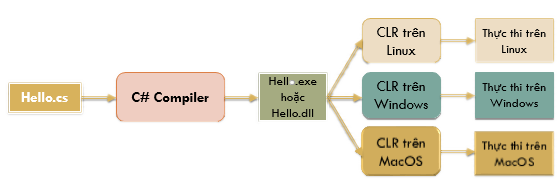
\includegraphics[scale=.4]{quatrinhthongdich.png}
		\end{center}
		\caption{Quá trình dịch chương trình trong C\#}		
	\end{figure}
\end{center}

C\# có thể tạo ra được nhiều loại ứng dụng, trong đó có 3 kiểu phổ biến được nhiều nhà lập trình viên sử dụng nhất đó là: Console, Window và ứng dụng Web. 

\subsection{Công cụ sinh dữ liệu thử Pex}
\subsubsection*{Giới thiệu}
Khái niệm về DSE và các ứng dụng sử dụng kỹ thuật DSE đã có từ lâu, nhưng Pex là một ứng dụng mỡ rộng hơn so với các phiên bản DSE trước. Trong Visual Stuio, Pex đã được tích hợp như một Add-in, và có thể tạo ra các test case kết hợp với các bộ kiểm thử khác nhau như NUnit và MSTest. 

Cũng như với Unit Test, ta có thể viết các lớp kiểm thử chứa các ca kiểm thử tham số hóa. Với sự hỗ trợ của Pex ta có thể thực thi các ca kiểm thử tham số hóa đó. Tuy nhiên không giống việc thực thi các lớp kiểm thử chứa các Unit Test, Pex chỉ thực thi được một ca kiểm thử tham số hóa trong mỗi lần chạy.

\lstinputlisting[caption = {Ca kiểm thử tham số sử dụng Pex}]{TestPex.cs}

\subsubsection*{Lọn chọn đầu vào kiểm thử với Pex}
Để có thể sinh các đầu vào cụ thể cho các tham số Unit test, Pex cần phải phân tích chương trình với các tham số kiểm thử này. Có 2 kỹ thuật phân tích chương trình đó là:

\begin{itemize}
	\item Phân tích tĩnh (static analysis): Kiểm chứng một tính chất nào đó của chương trình bằng việc phân tích tất cả các đường đi thực thi. Kỹ thuật này coi các cảnh bảo (violations) là các lỗi (error).
	\item Phân tích động (dynamic analysis): Kiểm chứng một tính chất bằng việc phân tích một số đường đi thực thi. Đây là một kỹ thuật phân tích động hỗ trợ việc phát hiện ra các lỗi (bugs) nhưng không khẳng định được rằng có còn những lỗi khác hay không. Các kỹ thuật này thường không tìm ra được tất cả các lỗi.
\end{itemize}

Pex cài đặt một kỹ thuật phân tích chương trình bằng cách kết hợp cả hai kỹ thuật phân tích chương trình ở trên gọi là DSE \cite{xie2009fitness, godefroid2005dart}. Về bản chất Pex là một công cụ hỗ trợ kỹ thuật kiểm thử hộp hắng (white-box testing). Tương tự như kỹ thuật phân tích chương trình tĩnh, Pex chứng minh được rằng một tính chất được kiểm chứng trong tất cả các đường đi khả thi. Pex chỉ báo cáo (reporting) về các lỗi thực sự như với kỹ thuật phân tích chương trình động.

Pex sử dụng bộ xử lý ràng buộc Z3 \cite{de2008z3} kết hợp với các lý thuyết toán học khác như hàm chưa định nghĩa, lý thuyết mảng, bit-vetor \cite{kroening2016decision} để giải quyết ràng buộc sinh ra trong quá trình thực thi tượng trưng động và sinh ra các đầu vào kiểm thử cụ thể cho tham số kiểm thử.

\subsubsection*{Mô hình ứng dụng Pex}
\begin{center}
	\begin{figure}[h]
		\begin{center}
			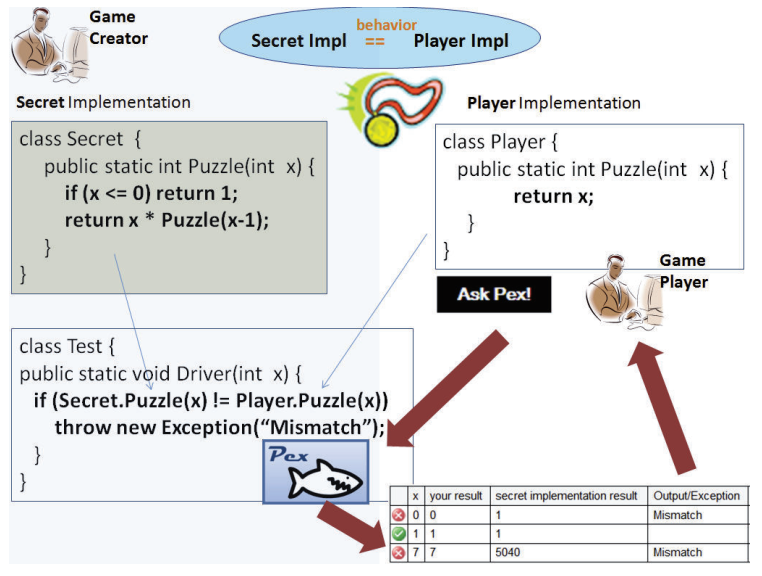
\includegraphics[scale=.4]{pex.png}
		\end{center}
		\caption{Mô hình ứng dụng Pex}
		
	\end{figure}
\end{center}

\section{Đánh giá kết quả thực nghiệm}
Nội dung Chương 2 và Chương 3 đã trình bày một số lý thuyết về kiểm thử phần mềm, các kỹ thuật sinh dữ liệu thử nghiệm, và các kỹ thuật đo độ tương tự hành vi chương trình \textbf{RS, SSE, PSE}. Áp dụng những lý thuyết trên, tôi thực nghiệm bằng cách xây dựng một ứng dụng, mô tả quá trình hoạt động của các kỹ thuật đo, và đánh giá kết quả các kỹ thuật đo, kết quả thực nghiệm đạt được như sau:

\begin{center}
	\begin{figure}[h]
		\begin{center}
			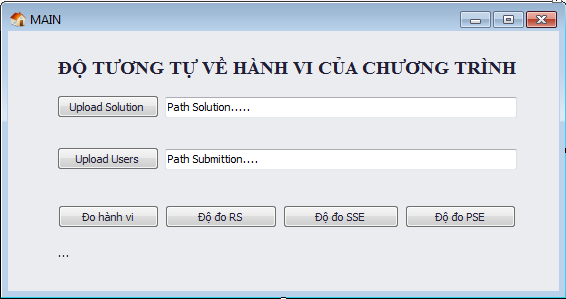
\includegraphics[scale=.5]{main.png}
		\end{center}
		\caption{Giao diện màn hình chính}		
	\end{figure}
\end{center}

Hai nút đầu tiên, cho phép chúng ta chọn file chương trình tham chiếu và files cần tính độ tương tự. Bên dưới là các chút chức năng đo hành vi, và tính toán độ tương tự hành vi của chương tình theo các độ đo khách nhau RS, SSE và PSE.

Một số files mẫu chương trình tham chiếu và chương trình cần tính độ tương tự (chương trình của sinh viên) có nội dung như sau:

\lstinputlisting[caption = {Chương trình tham chiếu}]{solution.cs}
\lstinputlisting[caption = {Chương trình của sinh viên thứ nhất}]{user1.cs}
\lstinputlisting[caption = {Chương trình của sinh viên thứ hai}]{user2.cs}

\subsection{Kết quả độ đo RS}
\begin{center}
	\begin{figure}[h]
		\begin{center}
			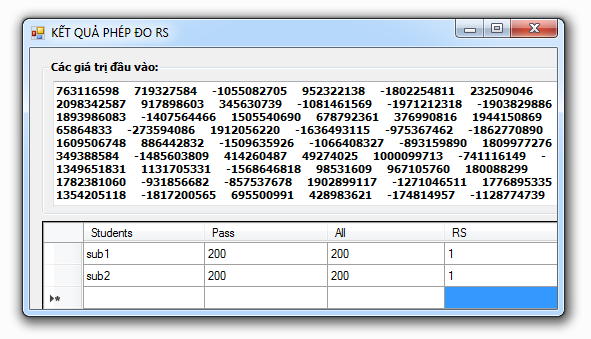
\includegraphics[scale=.5]{kq_rs.png}
		\end{center}
		\caption{Kết quả độ đo RS}		
	\end{figure}
\end{center}

Dựa vào kết quả độ đo RS ở trên, chúng ta có danh sách các giá trị đầu vào được sinh ngẫu nghiên từ miền giá trị đầu vào của các chương trình. Hai chương trình của sinh viên được đánh giá là tương đương với chương trình tham chiếu và đều có kết quả là 1. Trong khi đó, điều kiện của Chương tình tham chiếu $(case 2: y += 8; break;)$, cấu trúc điều kiện của sinh viên thứ nhất $(case 2: y += 8; break;)$, cấu trúc điều kiện của sinh viên thứ hai $(if (x == 2) return y *= 4;)$ và $(if (x == 3) return y *= 6;)$, mã lệnh của hai sinh viên đều có hành vi khác biệt so với Chương trình tham chiếu. Kết quả độ đo \textbf{RS} cho kết quả ở mức tương đối, giá trị thử nghiệm không phủ hết các trường hợp chương trình có khả năng thực thi.

\subsection{Kết quả độ đo SSE}
\begin{center}
	\begin{figure}[h]
		\begin{center}
			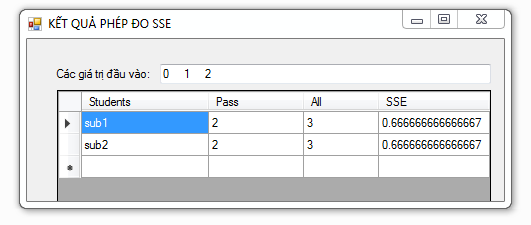
\includegraphics[scale=.5]{kq_sse.png}
		\end{center}
		\caption{Kết quả độ đo SSE}		
	\end{figure}
\end{center}

Phân tích Chương trình tham chiếu với kỹ thuật DSE chúng ta có các giá trị đầu vào thử nghiệm lần lượt là $0, 1, 2$. Các giá trị đầu vào thử nghiệm này khi thực thi trên chương trình của hai sinh viên cho 2 kết quả đầu giống nhau trên tổng số 3 kết quả so với chương trình tham chiếu, đạt tỷ lệ $0,66$. Kết quả độ đo SSE cho chúng ta một kết quả chính xác hơn kết quả độ đo RS. Những phép đo SSE lại khi không xem xét các hành vi trong chương trình của sinh viên, không tạo ra được các giá trị đầu vào thử nghiệm có khả năng phủ hết các nhánh trong Chương trình của sinh viên. Trong khi Chương trình của sinh viên hiện có hành vi khác biệt so với Chương trình tham chiếu.

\subsection{Kết quả độ đo PSE}
\begin{center}
	\begin{figure}[h]
		\begin{center}
			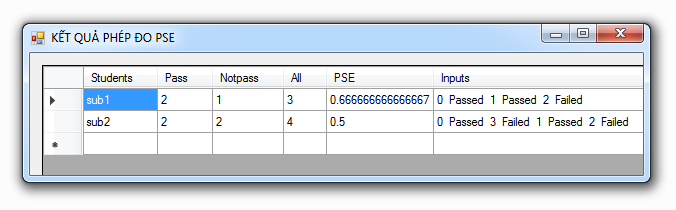
\includegraphics[scale=.5]{kq_pse.png}
		\end{center}
		\caption{Kết quả độ đo PSE}		
	\end{figure}
\end{center}

Kết quả độ đo PSE đã thay đổi so với kết quả độ đo SSE. PSE tạo ra $4$ giá trị đầu vào thử nghiệm trên Chương trình kết hợp giữa Chương trình tham chiếu và Chương trình của sinh viên thứ $2$, lần lượt là $0, 1, 2, 3$. Kết quả phép đo PSE cho sinh viên thứ nhất đạt $0.66$, và kết quả phép đo PSE của sinh viên thứ hai đạt $0,5$, kết quả này chính xác nếu chúng ta so sánh với việc phân tích thủ công. Các giá trị thử nghiệm đáp ứng được mục tiêu phủ hết các nhánh của Chương trình cần tính và Chương tình tham chiếu.

\section{Khả năng ứng dụng}
Các kỹ thuật đo độ tương tự trình bày trong đề tài này có thể áp dụng được trong nhiều lĩnh vực, nhưng chủ yếu tập trung vào giáo dục, các chương trình đào tạo lập trình viên, hay đào tạo kỹ sư phần mềm... Một số ứng dụng thực tế có thể phát triển trong tương lai như: 

\textbf{\textit{Đánh giá tiến bộ trong lập trình:}} Theo dõi sự tiến bộ trong học tập là một việc quan trọng, mà ngay cả với giảng viên và sinh viên. Có nhiều tiêu chí đánh giá sự tiến bộ trong học tập của sinh viên, trong đó tiêu chí về điểm số là một trong những tiêu chí cơ bản nhất. Một bảng điểm thống kê điểm số, thành tích học tập của sinh viên sẽ thể hiện được sự tiến bộ của sinh viên trong học tập. Một ứng dụng hỗ trợ chấm điểm, lưu trữ, thống kê và đánh giá điểm số của sinh viên là sẽ là một công cụ hỗ trợ đắc lực cho giảng viên trong công tác quản lý của mình. Nếu số liệu thống kê kết quả các bài kiểm tra của sinh viên ngày càng cao, chứng tỏ sinh viên nắm được nội dung và kiến thức của chương trình đào tạo, và kết quả tốt sẽ là một động lực giúp cho sinh viên thêm tự tin, đam mê công việc học tập của mình. Ngược lại, nếu một sinh viên có điểm số ngày càng thấp đi, chứng tỏ sinh viên đang có vấn đề trong kiến thức của của mình, lúc này tốt nhất sinh viên nên dừng lại và kiểm tra xem vấn đề mình đang gặp phải. 

\textit{\textbf{Xếp hạng tự động:}} Công việc chấm điểm, phân loại và xếp hạng các bài kiểm tra của sinh viên cũng là một công việc tốn không ít công sức của giảng viên. Để giảm bớt gánh nặng cho giảng viên, chúng ta có thể sử dụng kết quả các phép đo trên từng bài tập của sinh viên như một phương pháp hỗ trợ công việc chấm điểm của từng sinh viên. Sự giống nhau về hành vi giữa Chương trình của sinh viên và Chương trình tham chiếu có thể là một yếu tố để phân loại sinh viên. Độ tương tự càng cao thì điểm số càng cao, các chỉ số này dựa hoàn toàn trên ngữ nghĩa của chương trình. Cách tiếp cận này giải quyết được các giới hạn trong trường hợp Chương trình của sinh viên giống với chương trình tham chiếu, nhưng khác nhau về ngữ nghĩa. Các kết quả trong việc xếp hạng tự động sẽ giúp tiết kiệm được thời gian và giảng viên có thể đưa ra giải pháp giúp những sinh viên có điểm số thấp khắc phục được hạn chế đang gặp phải.

\textit{\textbf{Gợi ý giải pháp lập trình:}} Thông thường, sinh viên thường viết code mới thực hiện chạy chương trình, lúc này sinh viên mới biết được kết quả đoạn code vừa thực hiện. Để hỗ trợ sinh viên viết code được tốt hơn, nếu như có một công cụ hỗ trợ kiểm tra theo thời gian thực và gửi thông báo lỗi nếu sinh viên viết code sai cú pháp hoặc chương trình bị lỗi không thể thực thi được. Ngoài ra, công cụ sẽ gợi ý giải pháp lập trình cho sinh viên bằng hình thức tự động tính toán thông báo kết quả các tham số đầu vào và đầu ra của chương trình so với chương trình được tham chiếu, đưa ra các số liệu về độ tương tự hành vi của chương trình.	

\subsection{Hướng phát triển}
Qua quá trình nghiên cứu và triển khai thực nghiệm, trong tương lai đề tài hướng tới phát triển thành một một ứng dụng hoàn chỉnh với việc bổ sung và hoàn thiện một số chức năng như sau:
\begin{itemize}
	\item Phát triển ứng dụng có thể chạy trên Web	
	\item Quản lý kết quả học tập sinh viên
	\item Thêm chức năng đánh giá, xếp hạng tự động
	\item Thêm chức năng gợi ý giải pháp lập trình
	\item Cải tiến các độ đo để cho kết quả tốt hơn và nhanh hơn
	\item Phát triển thêm các nền tảng lập trình khác như Java, C++..		
\end{itemize}

\section{Kết luận}
Qua quá trình nghiên cứu đề tài, có thể thấy rằng việc phát triển và ứng dụng các kỹ thuật đo đang dần trở nên phổ biến trong các chương trình giáo dục và đào tạo lập trình viên online. Những lợi ích, hiểu quả của việc đánh giá độ tương tự hành vi mang lại là rất thiết thực. Các kỹ thuật này không chỉ giúp quá trình giảng dạy của giảng viên được thuận lợi hơn, tiết kiệm được thời gian cũng như công sức trong công tác quản lý. Ngoài ra, sinh viên có được một môi trường tốt để tự rèn luyện, nâng cao các kỹ năng lập trình của bản thân. Việc tạo động lực giúp sinh viên có sự hứng thú và đam mê lập trình là rất cần thiết. Một khi sinh viên có tư duy và kỹ năng lập trình tốt, sinh viên sẽ tự tin vào năng lực của bản thân để tiếp tục phát phát triển sự nghiệp sau khi ra trường.

Đề tài đã thực hiện nghiên cứu nhiều vấn đề, như nghiên cứu kiểm thử phần mềm, sinh ngẫu nhiên dữ liệu thử, hay kỹ thuật DSE một kỹ thuật được ứng dụng trong công cụ PEX của Microsoft để giải quyết các ràng buộc sinh ra các tham số đầu vào thử nghiệm có độ phủ cao, nghiên cứu các phép đo RS, SSE, PSE để đo độ tương tự hành vi của chương trình. Trên cơ sở lý thuyết các kỹ thuật đo, xây dựng một công cụ để minh họa cho các phép đo. Kết quả của các phép đo là tương đối tốt, tạo ra nhiều hướng phát triển trong tương lai.

Trong quá trình thực hiện đề tài, bản thân tôi cũng gặp phải rất nhiều khó khăn như: Lượng kiến thức cơ sở cần phải nghiên cứu để triển khai thực hiện đề tài rất nhiều; cùng với đó là kinh nghiệm của bản thân tôi trong việc thực hiện các đề tài chưa có. Tuy nhiên, với sự động viên và tận tình giúp đỡ của giáo viên hướng dẫn, đề tài đã đạt được mục tiêu đề ra, có thể mở ra nhiều hướng nghiên cứu và phát triển khác của đề tài như cải tiến các kỹ thuật đo, kết hợp với kỹ thuật DSE để có kết quả các phép được chính xác hơn, nhạy hơn. Tiếp tục nghiên cứu, phát triển trên các ngôn ngữ khác như Java, C++ ... và chạy được trên nhiều nền tảng PC, Web. 

